\documentclass[openany]{article}

%Typesetting and language
\usepackage[american]{babel}
\usepackage[T1]{fontenc}
\usepackage{charter}
\usepackage{enumitem}
\usepackage{hyperref}

%Symbols
\usepackage{amssymb, amsmath, amsthm, bm}
\usepackage{mathrsfs}
\usepackage{mathtools}
\usepackage{marvosym}
\usepackage{MnSymbol}

%Colors & graphics
\usepackage[dvipsnames]{xcolor}
\usepackage{pgfplots}
\usepackage[numbered,framed]{matlab-prettifier}
\usepackage{pgfplots}
\usepackage{listings}
\usepackage{tikz}
\usetikzlibrary{arrows.meta}
\usepackage[object=vectorian]{pgfornament}
\usepackage{wrapfig}
\usepackage{varwidth}
\usepackage[framemethod=TikZ]{mdframed}
\usepackage{caption}
\usepackage{float}
\usepackage{geometry}
\usepackage{ulem}
\usepackage[most]{tcolorbox}
\usepackage{array}

\setlength{\parindent}{0pt}

\makeatletter
\g@addto@macro\bfseries{\boldmath}
\makeatother


\renewcommand{\Re}{\mathfrak{Re}}
\renewcommand{\Im}{\mathfrak{Im}}

\geometry{left=2cm,right=2cm,bottom=2cm,top=2cm}

\usepackage{fancyhdr}
\pagestyle{fancy}
\fancyhf{}
\renewcommand{\sectionmark}[1]{\markright{\arabic{section} - #1}}
\cfoot{\thepage}
\lhead{Algo Learning}
\chead{Dynamic Programming}
\rhead{Adam Yang}
\renewcommand{\headrulewidth}{1pt}


\DeclareMathOperator{\sgn}{sgn}
\DeclareMathOperator{\im}{im}
\DeclareMathOperator{\var}{var}
\DeclareMathOperator{\Orb}{Orb}
\DeclareMathOperator{\Fix}{Fix}
\DeclareMathOperator{\Stab}{Stab}
\DeclareMathOperator{\cov}{cov}
\DeclareMathOperator*{\esssup}{ess\,sup}
\DeclareMathOperator{\corr}{corr}
\DeclareMathOperator{\lik}{lik}
\DeclareMathOperator*{\argmin}{argmin}
\DeclareMathOperator*{\argmax}{argmax}

\newcommand{\niceline}[2]{%
		\nointerlineskip \vspace{.5\baselineskip}\hspace{\fill}
		{\color{#1}
				\resizebox{0.5\linewidth}{2ex}
				{{%
								{\begin{tikzpicture}
										\node  (C) at (0,0) {};
										\node (D) at (9,0) {};
										\path (C) to [ornament=#2] (D);
										\end{tikzpicture}}}}}%
		\hspace{\fill}
		\par\nointerlineskip \vspace{.5\baselineskip}
}

\definecolor{darkViolet}{HTML}{9400D3}
\newcommand{\sweetline}{%
		\noindent
		\begin{center}
				{\color{darkViolet}
						\resizebox{0.5\linewidth}{1ex}
						{{%
										{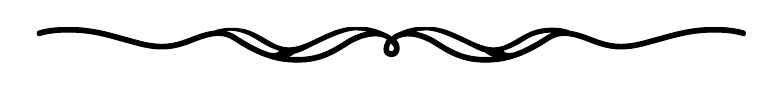
\begin{tikzpicture}
												\node  (C) at (0,0) {};
												\node (D) at (9,0) {};
												\path (C) to [ornament=85] (D);
												\end{tikzpicture}}}}}%
		\end{center}
}

\definecolor{remarkPurple}{HTML}{8346FF}
\definecolor{defBlue}{HTML}{0673FF}
\definecolor{exPurple}{HTML}{FF8710}

%THEOREM
\newtcbtheorem[auto counter,number within=section]{theorem}{Theorem}%
{enhanced,colback=white, breakable,frame empty,interior empty,colframe=cyan!50!white, top=8mm,
				coltitle=black,fonttitle=\bfseries,colbacktitle=cyan!15!white,
				borderline={0.5mm}{0mm}{cyan!15!white},
				borderline={0.5mm}{0mm}{cyan!50!white,dashed},
				attach boxed title to top left={yshift=-4mm},
				boxed title style={sharp corners=east,boxrule=1pt},varwidth boxed title}{thm}

%PROPOSITION
\newtcbtheorem[use counter from=theorem]{proposition}{Proposition}%
{enhanced,colback=white,breakable,frame empty,interior empty,colframe=defBlue!75!white, top=8mm,
				coltitle=black,fonttitle=\bfseries,colbacktitle=defBlue!20!white,
				borderline={0.5mm}{0mm}{defBlue!20!white},
				borderline={0.5mm}{0mm}{defBlue!50!white,dashed},
				attach boxed title to top left={yshift=-4mm},
				boxed title style={sharp corners=east,boxrule=1pt},varwidth boxed title}{prop}

%DEFINITION
\newtcbtheorem[use counter from=theorem]{definition}{Definition}%
{enhanced,colback=white,breakable,frame empty,interior empty,colframe=defBlue!75!white, top=8mm,
				coltitle=black,fonttitle=\bfseries,colbacktitle=defBlue!20!white,
				borderline={0.5mm}{0mm}{defBlue!20!white},
				borderline={0.5mm}{0mm}{defBlue!50!white,dashed},
				attach boxed title to top left={yshift=-4mm},
				boxed title style={sharp corners=east,boxrule=1pt},varwidth boxed title}{def}

%COROLLARY
\newtcbtheorem[use counter from=theorem]{corollary}{Corollary}%
{enhanced,colback=white,breakable,frame empty,interior empty,colframe=defBlue!75!white, top=8mm,
				coltitle=black,fonttitle=\bfseries,colbacktitle=defBlue!20!white,
				borderline={0.5mm}{0mm}{defBlue!20!white},
				borderline={0.5mm}{0mm}{defBlue!50!white,dashed},
				attach boxed title to top left={yshift=-4mm},
				boxed title style={sharp corners=east,boxrule=1pt},varwidth boxed title}{cor}

%REMARK
\newtcbtheorem[no counter]{remark}{Remark}%
{detach title, colback=white,enhanced ,breakable,frame empty, interior empty, fonttitle=\bfseries, coltitle=Violet, before upper={\tcbtitle.\quad},
				borderline west={0.5mm}{0mm}{remarkPurple!40!white},
				borderline west={0.5mm}{0mm}{remarkPurple!60!white,dashed}}{remark}

%LEMMA
\makeatletter
\newtcbtheorem[number within = tcb@cnt@theorem]{lemma}{Lemma}%
{enhanced,breakable,colback=white,frame empty,interior empty,colframe=orange!75!white, top=8mm,
				coltitle=black,fonttitle=\bfseries,colbacktitle=orange!20!white,
				borderline={0.5mm}{0mm}{orange!20!white},
				borderline={0.5mm}{0mm}{orange!50!white,dashed},
				attach boxed title to top left={yshift=-4mm},
				boxed title style={sharp corners=east,boxrule=1pt},varwidth boxed title}{lemma}
\makeatother


%PROOF
%%{enhanced,breakable,frame empty,interior empty,colframe=remarkPurple!75!white, top=8mm,
%	coltitle=black,fonttitle=\bfseries,colbacktitle=remarkPurple!20!white,
%	borderline={0.5mm}{0mm}{remarkPurple!20!white},
%	borderline={0.5mm}{0mm}{remarkPurple!50!white,dashed},
%	attach boxed title to top left={yshift=-4mm},
%	boxed title style={sharp corners=east,boxrule=1pt},varwidth boxed title}{prf}


\tcolorboxenvironment{proof}{% amsthm' 
				blanker,breakable,left=5mm,
				before skip=10pt,after skip=10pt,
				borderline west={0.5mm}{0pt}{cyan!40},
				borderline west={0.5mm}{0pt}{remarkPurple!10, dashed}}

%PROBLEM
\newtcbtheorem[auto counter]{problem}{Problem}%
{enhanced,breakable,colback=white,frame empty,interior empty,colframe=cyan!50!white, top=8mm,
				coltitle=black,fonttitle=\bfseries,colbacktitle=cyan!20!white,
				borderline={0.5mm}{0mm}{cyan!20!white},
				borderline={0.5mm}{0mm}{cyan!50!white,dashed},
				attach boxed title to top left={yshift=-4mm},
				boxed title style={sharp corners=east,boxrule=1pt},varwidth boxed title}{prob}

%EXAMPLE
%\newtcbtheorem[use counter from=problem]{example}{Example}%
%{enhanced,breakable,colback=white,frame empty,interior empty,colframe=remarkPurple!50!white, top=8mm,
%		coltitle=black,fonttitle=\bfseries,colbacktitle=remarkPurple!30!white,
%		borderline={0.5mm}{0mm}{remarkPurple!30!white},
%		borderline={0.5mm}{0mm}{remarkPurple!30!white,dashed},
%		attach boxed title to top left={yshift=-4mm},
%		boxed title style={sharp corners=east,boxrule=1pt},varwidth boxed title}{ex}


\newtcbtheorem[use counter from=theorem]{example}{Example}%
{detach title, colback=white,enhanced ,breakable,frame empty, interior empty, fonttitle=\bfseries, coltitle=black, before upper={\tcbtitle.\quad},
		borderline west={0.5mm}{0mm}{remarkPurple!30!white},
		borderline ={0.5mm}{0mm}{remarkPurple!30!white}}{example}

%SOLUTION
\newtcbtheorem[no counter]{solution}{Solution}%
{enhanced,breakable,colback=white,frame empty,interior empty,colframe=green!75!white, top=8mm,
				coltitle=black,fonttitle=\bfseries,colbacktitle=green!20!white,
				borderline={0.5mm}{0mm}{green!20!white},
				borderline={0.5mm}{0mm}{green!50!white,dashed},
				attach boxed title to top left={yshift=-4mm},
				boxed title style={sharp corners=east,boxrule=1pt},varwidth boxed title}{sol}
\definecolor{realPurple}{HTML}{AA05F9}
\definecolor{gray}{rgb}{0.5,0.5,0.5}
\definecolor{dkgreen}{rgb}{0,0.6,0}
\definecolor{mauve}{rgb}{0.58,0,0.82}

\lstset{frame=tb,
				style=Matlab-editor,
				language=C,
				aboveskip=3mm,
				belowskip=3mm,
				xleftmargin=3mm,
				showstringspaces=false,
				columns=flexible,
				frame=none,
				basicstyle={\small\ttfamily},
				numberstyle=\tiny\color{gray},
				keywordstyle=\color{blue},
				commentstyle=\color{dkgreen},
				stringstyle=\color{mauve},
				breaklines=true,
				breakatwhitespace=true,
				mlshowsectionrules = true,
				tabsize=3,
				backgroundcolor=\color{cyan!5}
}

\newcommand\mmybox[2][fill=cyan!20]{%
    \tikz[baseline]\node[%
        inner ysep=0pt, 
        inner xsep=2pt, 
        anchor=text, 
        rectangle, 
        rounded corners=1mm,
        #1] {\strut#2};%
}


\def\changemargin#1#2{\list{}{\rightmargin#2\leftmargin#1}\item[]}
\let\endchangemargin=\endlist

\linespread{1.4}



% MAIN DOC
\begin{document}

\title{Dynamic Programming}
\author{Adam Yang}
% \date{\today}
\maketitle




\section*{Problem1}

\subsection*{Algorithm}
\begin{proof}[Algorithm]{}
		\renewcommand{\qedsymbol}{}
		An Algorithm to calculate the sequence of die rolls gets to winning square as quickly as possible.
		\begin{lstlisting}[basicstyle=\fontsize{8}{9}\selectfont\ttfamily]
// this is a pseudo-code, for convenience we define add_square() for vector<T> similar to push_back() in C++. It returns an original list added with a new square at the end and won't impact original list
// push_back() is simply C++ push_back() method for vector<T>
vector<int> findSeq( int[] d )
{
    // define infinity as the largest number we can get
    // won't use INT_MAX for convenience (overflowing issue)
    // here we denote the size of d[] as n
    // Will explain the variables used in algorithm later
    // if i is a ladder, d[i] = j, j>i (j is the termination of i)
    // if i is a chute, d[i] = undefined
    // if i is a normal square, d[i] = i
    if(n <= 6) return {0, d[n]}; //trivially solved by rolling once
    struct square {
        int count; // count of times of rolls
        vector<int> seq; // quickest sequence to reach square i
    }
    // initialization
    vector<square> dp;
    dp.push_back( {0, {}} );
    for(int i = 1; i <= n; ++i) {
        if(i>=1 && i<=6 && d[i] != undefined) dp.push_back( {1, {i} } ) // roll once, sequence = {i}
        else dp.push_back( {infinity, {} } );
    }
    for(int i = 1; i <= 6; ++i) {
        if(d[i]>i) {
            dp[d[i]].count = 1;
            dp[d[i]].seq = dp[i].seq; // climb to d[i]
        }
    }
    // start finding sequence
    for(int i = 7; i <= n; ++i) {
        if(d[i] == undefined) continue;
        int min_predecessor_count = dp[i-6].count;
        int min_predecessor_index = i-6;
        for(int s = i-5; s <= i-1; ++s){
            if(dp[s].count < min_predecessor_count){ //find min count & index
                min_predecessor_count = dp[s].count
                min_predecessor_index = s;
            }
        }
        dp[i].count = min(min_predecessor+1, dp[i]);
        //notice that whenever we reach i, we either roll a dice from its 6 predecessor
        //or we have reached i through a ladder 1 <= k < i. if we reached i before, seq[i] = k, dp[i] != infinity. Denote i's predecessor's index as k if i has one. We can also simply find k by looking at the last element of dp[i].seq.back()
        if(dp[i].count < dp[min_predecessor_index].count + 1){ //it is cheaper to reach i through k
            //we do nothing since it has had a quickest sequence
        } else {
            dp[i].seq = dp[min_predecessor_index].seq.add_square(i); //add i since need to roll to i
        }
        
        if(d[i] > i) { // i is ladder
            dp[d[i]].count = min(dp[min_predecessor_index].count + 1, dp[d[i]].count);
            if(dp[min_predecessor_index].count+1 < dp[d[i]].count) { // we roll to i once from min_predecessor_index
                dp[d[i]].seq = dp[min_predecessor_index].seq; //don't need to add d[i] since we climb there
            }
        }
    }
    
    return dp[n].seq; //if dp[n].count == infinity or dp[n].seq.size() == 0, can't reach n
}
		\end{lstlisting} 
\end{proof}



\begin{proof}[Explanation]{}
		\renewcommand{\qedsymbol}{} % hide the QED square
        I'll explain some variable used in pseudo-code above here

        \textbf{int[] d:} this is an input array that the problem provides, d[i] stores the information for each square, as explained from line 3 to 7

        \textbf{struct square:} this is a collection of information for each square i, i$\in$[0,n]. \textbf{square.count} stores the how many times to get to i, \textbf{square.seq} stores the sequence of roll to get i. Notice that if we get i by climbing a ladder, we won't need to record i into the sequence since we only need the sequence of rolling dice.
        
        \textbf{vector<Square> dp:} dp[] needs n+1 elements since the map ranges from 0 to n (Don't consider the '/' char here since it's a pseudo-code). i $\in$ [0 , n], dp[i] stores two information through \texttt{struct square}. dp[i].count is the least times of rolling a dice to get i, dp[i].seq is the sequence of rolling a dice to get i. Notice that, for every i$\in$[0,n], if i is a chute, we simply skip them in the loop since we will never roll a dice to get to a chute and if we get to this chute through a ladder before, its information has been updated when we found the ladder, we will prove this later.
        
        \textit{Initialization:} \textbf{dp[0] = \{0,\{\}\}} because we start at 0. \textbf{For i=1,2,3,4,5,and 6,} we initialize dp[i].count = 1, dp[i].seq = \{i\} if they are not chutes since we can roll from 1-6 from starting point 0 and get to i and it takes indeed least step for i. \textbf{For the i$\in$[7:n],} we initialize dp[i].count = $\infty$ and dp[i].seq = \{\} since we haven't reach them before we start finding them. Then we look back to i=1,2,3,4,5,6, if i is a ladder, we also update dp[d[i]].count = 1 where d[i] is the destination of ladder i because they only take one roll to arrive i and then to d[i], dp[d[i]].seq = dp[i].seq because we only need to roll once to get to i and then d[i].

       
\end{proof}

\subsection*{Proof}
\begin{proof}[Correctness]{}
    For notation, count = $\infty$ and seq = \{\} are dummy values to denote a square has never been reached. For each square, it stores information about the count and seq that corresponds to each other. Saying the information for a square i is optimal simply means dp[i].seq is the sequence that takes least times of roll and dp[i].count stores the times of roll. First, let's prove some properties in the algorithm that we'll use in proof.
\subsubsection*{Property 1}
    For i$\in$[7,n], when we loop to check square i (starting from line 31), if we have reached i through some ladder k before, 1$\leq$k$<$i, d[k] = i, dp[d[k]] = dp[i] has stored some "count" of rolls and "seq" that take temporarily least rolls before we do comparison with i's 6 predecessor (count != $\infty$, seq != \{\}).
    \begin{proof}{Property 1}
         Observing the algorithm on line 35-37, 51-53, whenever we found a ladder k, we always take a look at its destination square, denoted as i, d[k] = i. There are two ways to reach i: (1) We have already reached i through some ladder k' before, 1$\leq$k'$<$i (2) We roll a dice from [k-6:k-1] to arrive i and climb to d[i]. This takes us min(dp[k-6:k-1].count) rolls plus another roll to i. Then, we do a comparison between (1) and (2) and update dp[i].count and dp[i].seq with the sequence that takes fewer times of roll. If it's the first time we reach i, dp[i].count = $\infty$ > min(dp[k-6:k-1].count)+1, dp[i] has stored the information that is temporarily optimal before we loop to i and check. If it's not the first time, we either replace square information with sequence taking fewer steps or and don't change the original information since it's better. Notice that in this case, dp[i].seq won't include i itself because we didn't roll to reach i.
         
         Since d[k] = i > k, whenever we loop to check i, we have already check k before (for loop property). Since we update the dp[d[k]] if k is a ladder, we have stored the optimal information for dp[d[k]] when we loop to d[k] before checking with d[k]'s 6 predecessor.
    \end{proof}

\subsubsection*{Property 2}
    For i$\in$[7,n], when we loop to check square i (starting from line 31), dp[i] will always store the information for the sequence with less times of roll when finishing checking.
    \begin{proof}
        Notice that we only have two ways to reach a square: roll a dice from its 6 predecessor or through some ladder 0 $\leq$ k $<$ i.
        (1) If i is a chute, the algorithm simply skip it since we will never roll a dice to reach a chute. Therefore, either we have reached i before through ladder k and the information for i has been updated when we reach k (Property 1), or we have never reached i and will never reach i and dp[i].count = $\infty$ dp.seq = \{\}.
        (2) If i is a ladder or a normal square, the algorithm compares its current reaching sequence rolling times with min(dp[i-6:i-1].count) + 1 and stores the better information on line 35 - 41. If we reach i through rolling once from its one of its 6 predecessors, the sequence will add i.
    \end{proof}

\subsubsection*{Property 3}
    The algorithm terminates.
    \begin{proof}
        Since the algorithm only use for loop on local variable i and s, all of which only have ++i or ++s operation on its value, the algorithm always terminates.
    \end{proof}

\begin{lemma*}{For i$\in$[7,n], when we finish checking i-1, i always store the optimal sequence information that takes least times of roll}
    

\end{lemma*}


Now, let's start proving the correctness.
For a optimal solution to reach a square i, either (1) we reach their by rolling a dice once from its 6 predecessor or (2) we reach their by climbing a ladder before

% \begin{center}
%     \texttt{OPT(i) := sequence of roll to reach i that takes least time of roll;
% \\OPT(i) = min( OPT(i-6)+\{i\}, OPT(i-5)+\{i\}, OPT(i-4)+\{i\}, \\OPT(i-3)+\{i\}, OPT(i-2)+\{i\}, OPT(i-1)+\{i\}, OPT$_{temp}$(i) );
% }
% \end{center}



    \textbf{Base Case:}
\end{proof}








\begin{theorem*}{}
    For DP, we often analyze relatively easy (or even trivial) properties of the optimum solution, and exploit them to derive an efficient algorithm
\end{theorem*}
\section*{Solution}
\begin{solution*}{}
    Define OPT(S):= maximum weight that can be obtained from intervals in S.

    \begin{center}
            \textbf{[Find the max from including interval i or not including i]}
    \end{center}
    
    OPT(S) = max( OPT(s\textbackslash \{i\}), w(i)+OPT(S \textbackslash \{everything intersecting i\}) )

    \textbf{Base Case:} OPT(\{\}) = 0

    \begin{proof}{This is not optimal if we do it recursively}
    
        Implementing this \textbf{recursively} is just exhaustive search with backtracking, and runs in about $2^n$ times.

        If we store all OPT(S) values in a table to avoid recomputing, with the current approach, we still take $2^n$ and the able size is $2^n$
    \end{proof}

    Our power is that we can choose the interval number i that we branch over. By a careful choice, we can make sure that only polynomially many (in fact: linearly many) subproblems need to solved.

    Assume from now on that intervals are sorted by non-decreasing finish time f(i). Subproblems of the form \{1,2,...,k\} for k = 0,...,n.

    We define the following notations
    
    OPT(k):= optimum weight for the subproblems \{1,2,...,k\}
    
    t(k):= the largest index j such that $f(j) < s(k)$ [the latest interval that does not intersect interval k.]
    
    Recurrence Relation:
    \[OPT(k) = max(OPT(k-1), w(k)+OPT(t(k)))\]

    \textbf{Base Case:} OPT(0) = 0
    
    \textbf{Justification:} The opt solution for intervals 1,..,k either doesn't contain k (in which case it is the OPT(k-1)) or it does contain k, and includes the opt solution for the still available intervals

    Final answer we're interested in: OPT(n)

    \textbf{Implementation:}

    \qquad \texttt{1. Sort intervals by non-decreasing f(i)}
    
    \qquad \texttt{2. Precompute all of the t[k];}
    
    \qquad \texttt{3. a[0] = 0;}
    
    \qquad \texttt{4. for(int i = 1; i <= n; ++i) a[i] = max(a[i-1], w[i]+a[t[i]]);}
    
    \qquad \texttt{5. return a[n];}

    To output the solution itself:
    \texttt{k=n; while(k>0) if (k yellow) {output k; k = t[k];} else k--;}
    

    
\end{solution*}

    \begin{proof}[\textbf{Running time}]{}
    \renewcommand{\qedsymbol}{}
    
        \qquad \texttt{1. O(nlogn)}
        
        \qquad \texttt{2. O(nlogn) with n binary searches, can improve to O(n)}
        
        \qquad \texttt{4. and return O(n)}
        
        \qquad \texttt{Other: O(1)}

        Total: O(nlogn)
    \end{proof}

    \begin{proof}[\textbf{Correctness Proof}]{}
    \renewcommand{\qedsymbol}{}
        We want to show that the algorithm outputs the right answer. Algorithm outputs a[n]; right answer is OPT(n). So we want to show that a[n]=OPT(n).

        
    \end{proof}



\section*{Problem}
\begin{problem*}{Edit Distance/Sequence Alginment}
    Given two strings x[1..n], y[1..m], how "similar"/"different" are they?

    \qquad 1. Hamming Distance: $\#$ of positions where the strings are different $\rightarrow$ not here (too easy)
    
    \qquad 2. Number or total cost of operations that turn x into y. (x$\rightarrow$y)
    
    \textbf{Operations:} insert - cost A; delete - cost A; replace - cost B [We could assign different costs for insertion and deletion, or for inserting/ deleting different characters, or for replacing different characters with
each other ==> nothing at all changes, just more parameters.]

    \textbf{Goal:} Given x, y, find a minimum cost sequence of operations that turns x into y.
\end{problem*}

\begin{proof}[Key Insight:]{}
		\renewcommand{\qedsymbol}{} % hide the QED square

        Alternative view: String alignment
        
        Insert blanks into one or both strings, and write them on top of each other. Cost of A for being matched with a blank, and B for being mismatched.

        \textbf{Goal:} find the min cost of insert blanks into both strings to minimize alignment cost

        What do we know about the optimum way of aligning x[1..n] with y[1..m]? It involves one of the following three:
        
        \qquad 1) x[n] is aligned with y[m]; incur cost B if x[n]!= y[m]. x[1..n-1] with y[1..m-1] are aligned *optimally*.
        
        \qquad 2) x[n] is aligned against a blank: incur cost A. x[1..n-1] and y[1..m] are aligned *optimally*.

        \qquad 3) y[m] is aligned against a blank: incur cost A. x[1..n] and y[1..m-1] are aligned *optimally*.

        \qquad Among these, the optimum solution (being optimal) chooses the better one.

        What makes this tick is that once we commit to including $i$, or to not including $i$, we compute/use the \textbf{*optimum*} solution for the resulting subproblem. \textbf{This is the key property for DP:} Any optimal soution must contain optimal solutions to the subproblems contained in it. We have to define the subproblems to that this is true, in order to be able to apply DP.
\end{proof}

\section*{Solution}
\begin{solution*}
    \textbf{Subproblems:} optimal alignment of the first i characters of x (for 0 $\leq$ i $\leq$ n) and the first j characters of y (for 0 $\leq$ j $\leq$ m).

    Define OPT(i,j) to be the minimum total cost for aligning x[1..i] with y[1..j].

    \textbf{Recurrence Relation:}
    
    OPT(i,j) = min(OPT(i-1,j-1) + B*[1 if x[i] != y[j]; 0 if x[i] = y[j]],OPT(i-1,j) + A, OPT(i,j-1) + A)

    \textbf{Base cases:}
    
OPT(i,0) = A*i [ turn length-i string into empty string]
OPT(0,j) = A*j [ turn empty string into length-j string]

    \textbf{Implementation:}

    \qquad \texttt{for (i = 0; i <= n; i++) a[i][0] = i*A;}

\qquad \texttt{for (j = 0; j <= m; j++) a[0][j] = j*A;}

\qquad \texttt{for (i = 1; i <= n; i ++)}

\qquad \qquad \texttt{for (j = 1; j <= m; j++)}

\qquad \qquad \qquad \texttt{if(x[i] == y[j]) a[i][j] = min(a[i-1][j-1], a[i-1][j] + A, a[i][j-1] + A);}

\qquad \qquad \qquad \texttt{else a[i][j] = min(a[i-1][j-1] + B, a[i-1][j] + A, a[i][j-1] + A);}

\qquad \texttt{return a[n][m];}
\end{solution*}

\begin{proof}{}{}
\textbf{To prove: a[n][m] = OPT(n,m)}

We will prove along the way: $\forall$ i, j: a[i][j] = OPT(i,j)

Proof by (strong) induction on \textbf{i+j}.

\textbf{Base case:} i+j = 0 => i = j = 0. a[0][0] = 0 = OPT(0,0).

\textbf{Induction Step:}

\textbf{Induction Hypothesis:} whenever i'+j' < i+j, a[i'][j'] = OPT(i',j')

\qquad \textbf{Case 1:} x[i] = y[j]:

Algorithm writes:\\ a[i][j] = min(a[i-1][j-1], a[i-1][j] + A, a[i][j-1] + A)\\= min (OPT(i-1,j-1), OPT(i-1,j) + A, OPT(i,j-1) + A)
[ by IH, because (i-1) + (j-1) < i+j, (i-1)+j < i+j, i+(j-1) < i+j ] = OPT(i,j) [ by recurrence relation ]

\qquad \textbf{Case 2:} x[i] != y[j], and i > 0 and j > 0

The algorithm writes:\\a[i][j] = min(a[i-1][j-1] + B, a[i-1][j] + A, a[i][j-1] + A) \\= min(OPT(i-1,j-1) + B, OPT(i-1,j) + A, OPT(i,j-1) + A) [ by IH ]
= OPT(i,j) [ by recurrence relation ]

\qquad \textbf{Case 3:} i = 0. The algorithm writes a[0][j] = A * j = OPT(0,j).

\qquad \textbf{Case 4:} j = 0. The algorithm writes a[i][0] = A * i = OPT(i,0).

\end{proof}
    
% \begin{proof}[Problem Insight]{}
% \renewcommand{\qedsymbol}{}
%         what do we know for sure about the opt solution set S, and on particular interval?

        
% \end{proof}

% END MAIN Doc
\end{document}
